\documentclass[10pt]{article}
\usepackage[a4paper, margin=2cm]{geometry}
%\usepackage{fullpage}
\usepackage[T1]{fontenc}
\usepackage[utf8]{inputenc}
\usepackage{graphicx}
\usepackage{mathpazo}
\pagenumbering{arabic}
\usepackage{siunitx}
\usepackage{amsmath}
\usepackage{mathtools} % Para poder usar "\Aboxed"
\usepackage{cancel} % Para usar "\cancel", de https://tex.stackexchange.com/questions/537955/how-do-cross-out-text-in-math-mode
\usepackage{multicol}
\usepackage[spanish]{babel}
\usepackage{steinmetz}
\DeclareSIUnit\voltampere{VA}
\DeclareSIUnit\var{VAr}
\setlength\parindent{0pt} % no indent

% Numbering pages on the right footer:
% (https://tex.stackexchange.com/questions/153167/how-to-set-page-number-at-right-footer)
\usepackage{fancyhdr}
% Turn on the style
\pagestyle{fancy}
\fancyhf{} % sets both header and footer to nothing
\renewcommand{\headrulewidth}{0pt} % To remove the top horizontal line created by default by "fancyhdr", from here: https://tex.stackexchange.com/questions/13896/how-to-remove-the-top-horizontal-bar-in-fancyhdr
% Set the right side of the footer to be the page number
\fancyfoot[R]{\thepage}


\usepackage{minibox} % Para poder partir el texto en 2 líneas usando "underbrace" u "overbrace", info aquí: https://tex.stackexchange.com/questions/8680/how-can-i-insert-a-newline-in-a-framebox


\usepackage{xparse} % For "overbrace/underbrace but with an arrow instead", from https://tex.stackexchange.com/questions/8720/overbrace-underbrace-but-with-an-arrow-instead

% Para poner flechas sobre los signos de igual, de aquí: https://tex.stackexchange.com/questions/8720/overbrace-underbrace-but-with-an-arrow-instead
\NewDocumentCommand{\overarrow}{O{=} O{\uparrow} m}{%
  \overset{\makebox[0pt]{\begin{tabular}{@{}c@{}}#3\\[0pt]\ensuremath{#2}\end{tabular}}}{#1}
}
\NewDocumentCommand{\underarrow}{O{=} O{\downarrow} m}{%
  \underset{\makebox[0pt]{\begin{tabular}{@{}c@{}}\ensuremath{#2}\\[0pt]#3\end{tabular}}}{#1}
}



\begin{document}

\large{\textbf{Ejercicio 7 de la colección de problemas}}

\vspace{3mm}
\large{\textbf{Enunciado}}:

\vspace{3mm}
Aplicar el método de los nudos en el circuito de la figura para
determinar:

\begin{enumerate}
    \item Los potenciales de los nudos A, B, C y D.
    \item Las intensidades de corriente señaladas.
    \item Carga, polaridad y energía almacenada en los condensadores, supuestos sin carga inicial.
\end{enumerate}

\begin{minipage}{0.85\linewidth}
  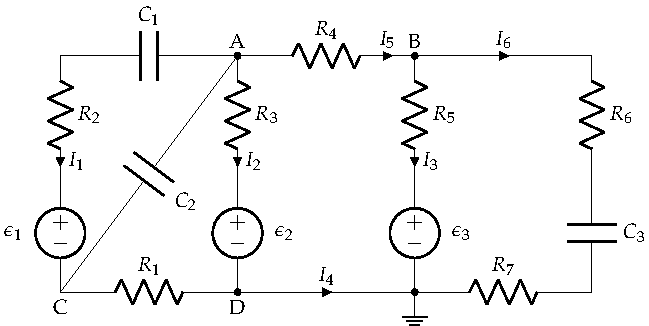
\includegraphics[scale=1.2]{figs/nudos_condensadores.pdf}
\end{minipage}
\begin{minipage}{0.25\linewidth}
    \textbf{Datos}:
    \vspace{2mm}
    
    $R_i = \qty[parse-numbers=false]{i}{\ohm}$\\
    $C_i = \qty[parse-numbers=false]{i}{\micro\farad}$\\
    $\epsilon_1=\qty{6}{\volt}$\\
    $\epsilon_2 = \qty{18}{\volt}$\\
    $\epsilon_3 = \qty{6}{\volt}$    
\end{minipage}

\vspace{7mm}

\hrulefill

\vspace{8mm}
\textbf{Solución}:
\vspace{4mm}

Sustituimos los condensadores por circuitos abiertos. En consecuencia, por las ramas correspondientes no puede circular corriente:

\vspace{2mm}
\begin{minipage}{0.75\linewidth}
  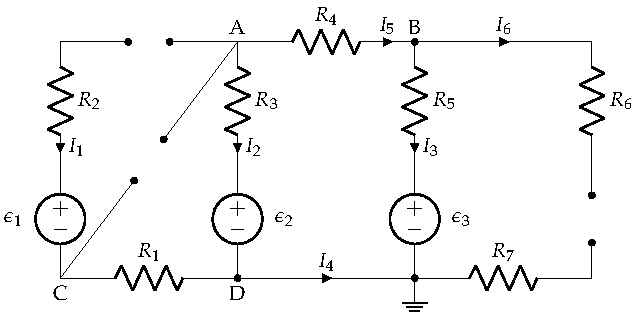
\includegraphics[scale=1.2]{figs/nudos_condensadores2.pdf}
\end{minipage}
\begin{minipage}{0.25\linewidth}
    \begin{align*}
      I_1 &= \qty{0}{\ampere}\\
      I_6 &= \qty{0}{\ampere}
    \end{align*}    
\end{minipage}

\vspace{6mm}

Luego el circuito equivalente es:

\begin{minipage}{0.32\linewidth}
    \begin{center}
        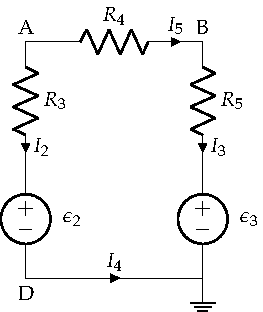
\includegraphics[scale=1.2]{figs/nudos_condensadores3.pdf}
    \end{center}
\end{minipage}
\begin{minipage}[c]{0.08\linewidth}
    \begin{center}
    $\LARGE \xrightarrow{\hspace*{0.5cm}}$ % https://latex.org/forum/viewtopic.php?t=3894
    \end{center}
\end{minipage}    
\begin{minipage}{0.6\linewidth}
    \begin{center}
        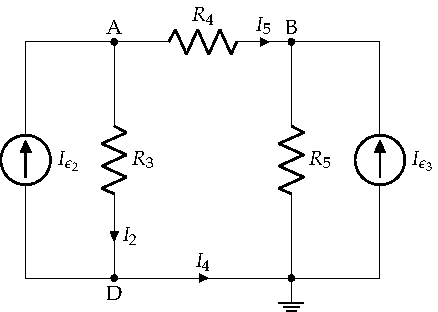
\includegraphics[scale=1.2]{figs/nudos_condensadores4.pdf}
    \end{center}
\end{minipage}

\vspace{6mm}

Donde hemos transformado las fuentes de tensión en fuentes de corriente, para poder aplicar el método de los nudos.

\vspace{3mm}
Formulando la ecuación general del método de los nudos:

\begin{equation*}
  \begin{bmatrix}
    G_3 + G_4 & -G_4\\
    -G_4 & G_5 + G_4\\
  \end{bmatrix} \cdot %
  \begin{bmatrix}
    U_A\\
    U_B
  \end{bmatrix} = %
  \begin{bmatrix}
    \epsilon_2/R_3\\
    \epsilon_3/R_5
  \end{bmatrix}
\end{equation*}

\vspace{4mm}
Sustituyendo valores y resolviendo:

\vspace{-5mm}
\begin{align*}
  U_A = \; \Aboxed{\qty{15}{\volt}}\\
  U_B = \; \Aboxed{\qty{11}{\volt}}
\end{align*}

Además, $U_D = \boxed{\qty{0}{\volt}}$ , dado que está conectado a tierra. Por otra parte, la caída de tensión en la resistencia $R_1$ es de $\qty{0}{\volt}$, dado que $I_1 = \qty{0}{\ampere}$, luego $U_C = U_D = \boxed{\qty{0}{\volt}}$.

\vspace{4mm}

Con estos resultados podemos obtener los valores de las corrientes de rama. Volvemos al circuito original para plantear las ecuaciones de rama:

\vspace{-4mm}
\begin{align*}
  U_A &= I_2 \cdot R_3 + \epsilon_2\\
  U_B &= I_3 \cdot R_5 + \epsilon_3
\end{align*}

\vspace{2mm}
De estas ecuaciones despejamos $I_2$ e $I_3$. Además, teniendo en cuenta que $I_1 = I_6 = \qty{0}{\ampere}$, tenemos:

\vspace{-3mm}
\begin{equation*}
  I_2 = I_4 = -I_3 = -I_5
\end{equation*}

Luego:

\begin{equation*}
  \boxed{I_1 = \qty{0}{\ampere}} \; , \quad
  \boxed{I_2 = \qty{-1}{\ampere}} \; , \quad
  \boxed{I_3 = \qty{1}{\ampere}} \; , \quad
  \boxed{I_4 = \qty{-1}{\ampere}} \; , \quad
  \boxed{I_5 = \qty{1}{\ampere}} \; , \quad
  \boxed{I_6 = \qty{0}{\ampere}}
\end{equation*}

\vspace{4mm}
Finalmente, calculamos las diferencias de potencial en los
condensadores. En $C_1$ asignamos la polaridad positiva en $A$, y
tenemos:

\begin{equation*}
  U_{AC} = U_{C_1} + \epsilon_1 \quad \rightarrow \quad U_{C_1} = \qty{9}{\volt}
\end{equation*}

\vspace{4mm}
Para $C_2$ y $C_3$, el cálculo es directo. Asignando polaridad positiva en $A$ y $B$, respectivamente:

\vspace{-3mm}
\begin{align*}
  U_{C_2} &=  U_{AC} = \qty{15}{\volt}\\
  U_{C_3} &=  U_{BD} = \qty{11}{\volt}
\end{align*}

\vspace{2mm}
En consecuencia, las cargas almacenadas en cada condensador son:

\vspace{-4mm}
\begin{align*}
  q_1 &= C_1 \cdot U_{C_1} = \boxed{\qty{9}{\micro\coulomb}}\\
  q_2 &= C_2 \cdot U_{C_2} = \boxed{\qty{30}{\micro\coulomb}}\\
  q_3 &= C_3 \cdot U_{C_3} = \boxed{\qty{33}{\micro\coulomb}}
\end{align*}

\vspace{1mm}
Y las energías almacenadas:

\vspace{-4mm}
\begin{align*}
  E_{C_1} &= \frac{1}{2} \cdot C_1 \cdot (U_{C_1})^2 = \boxed{\qty{40.5}{\micro\joule}}\\
  E_{C_2} &= \frac{1}{2} \cdot C_2 \cdot (U_{C_2})^2 = \boxed{\qty{225}{\micro\joule}}\\
  E_{C_3} &= \frac{1}{2} \cdot C_3 \cdot (U_{C_3})^2 = \boxed{\qty{181.5}{\micro\joule}}
\end{align*}

\end{document}
